% =====================================================================
% TC-MIL conference talk. Clean modern deck on the metropolis theme.
% Compile: pdflatex presentation.tex  (twice, for the title/section refs)
% Reuses the paper's figure PDFs (fig_calibration, fig3_faithfulness).
% =====================================================================
\documentclass[10pt,aspectratio=169]{beamer}

\usetheme{metropolis}
\metroset{sectionpage=progressbar, numbering=fraction, progressbar=foot}

\usepackage{booktabs}
\usepackage{amsmath}
\usepackage{xcolor}
\usepackage{tikz}
\usetikzlibrary{positioning, fit, arrows.meta}
\usepackage{pgfplots}
\pgfplotsset{compat=1.16}
\usepackage{multirow}
% mean$\pm$std with [CI], reused verbatim from the paper tables
\newcommand{\celld}[3]{\shortstack{#1{\footnotesize\,$\pm$#2}\\[-1.5pt]{\tiny[#3]}}}

% --- restrained, professional accent palette -------------------------
\definecolor{mDarkTeal}{HTML}{1F4E5F}
\definecolor{mAccent}{HTML}{0E7C7B}
\definecolor{mGood}{HTML}{2E7D32}
\definecolor{mWarn}{HTML}{B23A48}
\setbeamercolor{frametitle}{bg=mDarkTeal}
\setbeamercolor{progress bar}{fg=mAccent}
\setbeamercolor{alerted text}{fg=mAccent}

\newcommand{\good}[1]{\textcolor{mGood}{#1}}
\newcommand{\bad}[1]{\textcolor{mWarn}{#1}}
\newcommand{\num}[1]{\textbf{#1}}

% --- keep appendix/backup frames out of the total slide count --------
% Final main-talk frame fixes \inserttotalframenumber; backups then
% re-show that same number, so the footer reads N/N, not N/(N+backups).
\newcommand{\backupbegin}{%
  \newcounter{framenumberappendix}%
  \setcounter{framenumberappendix}{\value{framenumber}}%
}
\newcommand{\backupend}{%
  \addtocounter{framenumberappendix}{-\value{framenumber}}%
  \addtocounter{framenumber}{\value{framenumberappendix}}%
}

% --- title -----------------------------------------------------------
\title{TC-MIL: Topic-Chunk Multiple-Instance Learning}
\subtitle{Text-only depression detection on DAIC-WOZ, under a leakage-free protocol}
\author{Saverio Napolitano, Biagio Carpaneto}
\date{}

\begin{document}

\maketitle

\begin{frame}{In one slide}
  \begin{itemize}
    \item \textbf{Task.} Detect depression from clinical-interview \emph{transcripts} (DAIC-WOZ).
    \item \textbf{Idea.} Make each MIL instance a short \emph{dialogue chunk}, not a single turn.
    \item \textbf{Result.} Single model: macro-F1 \num{0.774}, micro-F1 \num{0.814}, ROC-AUC \num{0.864}
          --- beats the cleanest verified baseline, matches the best reported single model.
    \item \textbf{What sets it apart.} A \emph{leakage-free} protocol, an explicit
          interviewer-prompt bias control, measured attention faithfulness, and honest negative results.
  \end{itemize}
  \begin{alertblock}{Thesis}
    A simple representation change, rigorously evaluated, beats the heavier MIL architectures we compare against.
  \end{alertblock}
\end{frame}

% =====================================================================
\section{The problem}

\begin{frame}{Two problems hold back text-only DAIC-WOZ}
  \begin{columns}[T]
    \begin{column}{0.5\textwidth}
      \textbf{1. A representation bottleneck}
      \begin{itemize}
        \item Prior systems classify \emph{single turns}.
        \item Most turns are backchannels: ``yeah'', ``mhm'', ``i don't know''.
        \item A frozen encoder maps these to near-identical vectors.
        \item \bad{Pooling cannot reliably recover information absent from the instance representation.}
      \end{itemize}
    \end{column}
    \begin{column}{0.5\textwidth}
      \textbf{2. An evaluation-protocol problem}
      \begin{itemize}
        \item Numbers leak via test-tuned thresholds,
        \item pooled cross-validation that shares subjects,
        \item the \emph{positional} interviewer-prompt shortcut (Burdisso et al.):
              keying on the late interview region where the mental-health questions
              sit $\Rightarrow$ macro-F1 0.90.
        \item \bad{Reported numbers are hard to trust and to compare.}
      \end{itemize}
    \end{column}
  \end{columns}
\end{frame}

% =====================================================================
\section{The method: TC-MIL}

\begin{frame}{The idea: a chunk restores context}
  \begin{columns}[c]
    \begin{column}{0.46\textwidth}
      \begin{itemize}
        \item Instance $=$ a short \emph{sliding window of dialogue} ($w{=}4$, stride $2$).
        \item $\approx$28 instances/interview, $\approx$65 words each.
        \item A window holds \emph{a question and its answer} --- restoring the context a
              single backchanneled turn lacks.
        \item[$\Rightarrow$] near-degenerate instances become \good{discriminative}.
      \end{itemize}
    \end{column}
    \begin{column}{0.54\textwidth}
      \resizebox{\linewidth}{!}{%
      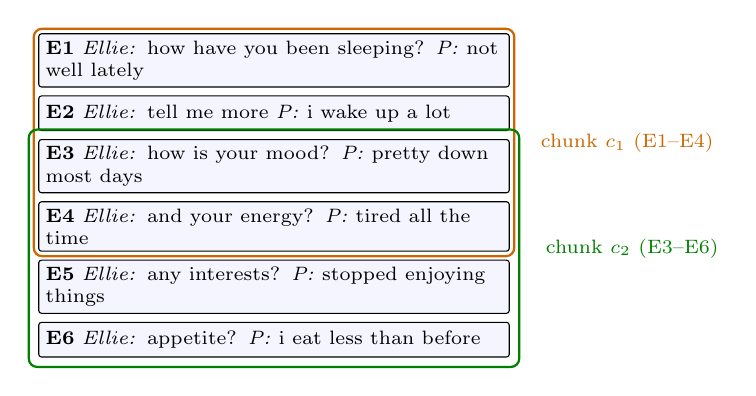
\begin{tikzpicture}[
        font=\scriptsize,
        ex/.style={draw, rounded corners=1pt, text width=58mm, align=left, inner sep=2.5pt, fill=blue!4, minimum height=4.4mm},
      ]
        \node[ex] (e1) {\textbf{E1} \emph{Ellie:} how have you been sleeping? \emph{P:} not well lately};
        \node[ex, below=1.0mm of e1] (e2) {\textbf{E2} \emph{Ellie:} tell me more \emph{P:} i wake up a lot};
        \node[ex, below=1.0mm of e2] (e3) {\textbf{E3} \emph{Ellie:} how is your mood? \emph{P:} pretty down most days};
        \node[ex, below=1.0mm of e3] (e4) {\textbf{E4} \emph{Ellie:} and your energy? \emph{P:} tired all the time};
        \node[ex, below=1.0mm of e4] (e5) {\textbf{E5} \emph{Ellie:} any interests? \emph{P:} stopped enjoying things};
        \node[ex, below=1.0mm of e5] (e6) {\textbf{E6} \emph{Ellie:} appetite? \emph{P:} i eat less than before};
        \node[draw=orange!80!black, thick, rounded corners=3pt, fit=(e1)(e4), inner sep=1.6pt] (w1) {};
        \node[draw=green!50!black, thick, rounded corners=3pt, fit=(e3)(e6), inner sep=3.4pt] (w2) {};
        \node[orange!80!black, anchor=west] at ([xshift=2mm]w1.east) {chunk $c_1$ (E1--E4)};
        \node[green!50!black, anchor=west] at ([xshift=2mm]w2.east) {chunk $c_2$ (E3--E6)};
      \end{tikzpicture}}
      \\{\scriptsize Overlapping windows ($w{=}4$, $s{=}2$). Text synthetic.}
    \end{column}
  \end{columns}
\end{frame}

\begin{frame}{Architecture --- intentionally minimal}
  \begin{center}
  \resizebox{\textwidth}{!}{%
  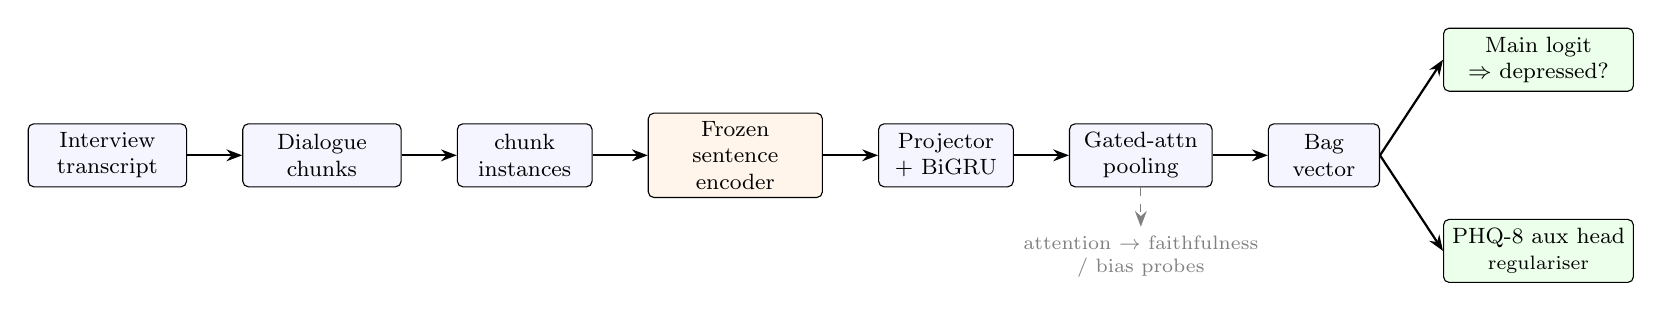
\begin{tikzpicture}[
    node distance=5mm and 7mm, font=\footnotesize,
    box/.style={draw, rounded corners=2pt, align=center, minimum height=8mm, inner sep=3pt, fill=blue!4},
    enc/.style={box, fill=orange!8},
    head/.style={box, fill=green!8},
    >={Stealth[length=2mm]}, arr/.style={->, thick},
  ]
    \node[box, text width=18mm] (interview) {Interview\\transcript};
    \node[box, right=of interview, text width=18mm] (chunk) {Dialogue\\chunks};
    \node[box, right=of chunk, text width=15mm] (inst) {chunk\\instances};
    \node[box, right=of inst, enc, text width=20mm] (encoder) {Frozen sentence\\encoder};
    \node[box, right=of encoder, text width=15mm] (proj) {Projector\\$+$ BiGRU};
    \node[box, right=of proj, text width=16mm] (attn) {Gated-attn\\pooling};
    \node[box, right=of attn, text width=12mm] (bag) {Bag\\vector};
    \node[head, above right=4mm and 8mm of bag, text width=22mm] (main) {Main logit\\$\Rightarrow$ depressed?};
    \node[head, below right=4mm and 8mm of bag, text width=22mm] (aux) {PHQ-8 aux head\\{\scriptsize regulariser}};
    \draw[arr] (interview) -- (chunk);
    \draw[arr] (chunk) -- (inst);
    \draw[arr] (inst) -- (encoder);
    \draw[arr] (encoder) -- (proj);
    \draw[arr] (proj) -- (attn);
    \draw[arr] (attn) -- (bag);
    \draw[arr] (bag.east) -- (main.west);
    \draw[arr] (bag.east) -- (aux.west);
    \node[below=5mm of attn, gray, font=\scriptsize, align=center] (interp) {attention $\to$ faithfulness\\/ bias probes};
    \draw[->, dashed, gray] (attn.south) -- (interp.north);
  \end{tikzpicture}}
  \end{center}
  \begin{itemize}
    \item Frozen encoder (\texttt{bge-large-en-v1.5}) $\Rightarrow$ embeddings pre-computed and cached.
    \item Gated-attention pooling over an optional residual BiGRU context; PHQ-8 aux head regularises.
    \item Head only $\sim\!10^5$ parameters --- \good{no mixup / focal / SWA / diversity losses}.
          Power is in the \emph{instance definition}, not a heavy network.
  \end{itemize}
\end{frame}

% =====================================================================
\section{Evaluating it honestly}

\begin{frame}{A leakage-free protocol}
  Every number in this talk obeys the same rules:
  \begin{itemize}
    \item Official AVEC2017 test split --- \emph{one} evaluation, never used to select.
    \item Per-seed mean $\pm$ std over \num{30} seeds (not a lucky single run).
    \item An \emph{a-priori prevalence} threshold: uses the model's scores and a
          training prior, \good{never a test label}.
    \item Subject-level bootstrap CIs $+$ non-parametric and parametric significance tests.
  \end{itemize}
\end{frame}

\begin{frame}{Headline result --- official test split}
  \begin{table}
    \centering\footnotesize
    \begin{tabular}{@{}lccc@{}}
      \toprule
      \textbf{Method} & \textbf{macro-F1} & \textbf{micro-F1} & \textbf{ROC-AUC} \\
      \midrule
      HAN+L (2020), single run               & 0.70 & --- & --- \\
      Bi-LSTM+Attn (2022), single run        & 0.783 & --- & --- \\
      Agarwal MV-IA (2022), single run       & 0.732 & 0.717 & --- \\
      Milintsevich (2023), verified baseline & 0.739{\scriptsize$\pm$.025} & 0.766{\scriptsize$\pm$.023} & --- \\
      Agarwal multi-view (2024), single run  & 0.80  & --- & --- \\
      \midrule
      \textbf{TC-MIL (ours)}
        & \celld{\good{\num{.774}}}{.029}{.591,.898}
        & \celld{\good{\num{.814}}}{.024}{.66,.92}
        & \celld{\good{\num{.864}}}{.011}{.751,.963} \\
      \bottomrule
    \end{tabular}
  \end{table}
  {\scriptsize TC-MIL cells: 30-seed per-seed mean$\pm$std (top) and subject-level
   bootstrap 95\% [CI] (bottom, 2000 resamples of the 47 test subjects).
   Milintsevich: per-seed mean$\pm$std (5 seeds). Other baselines: single run, no std or interval reported.}
  \begin{itemize}
    \item Beats the cleanest \emph{verified} baseline on every reported metric
          ($p=3.8\times10^{-7}$, one-sample $t$ over 30 seeds).
    \item Matches the best reported single models \emph{within one seed std} ---
          they report a single run, no AUC, no bias control, no interval.
  \end{itemize}
\end{frame}

% =====================================================================
\section{Why it works}

\begin{frame}{The architecture ladder localises the gain}
  Same protocol, full lineage retrained from scratch (official split, 30-seed mean$\pm$std):
  \begin{table}
    \centering\small
    \begin{tabular}{@{}lcc@{}}
      \toprule
      \textbf{Architecture} & \textbf{macro-F1} & \textbf{ROC-AUC} \\
      \midrule
      dialogue mean (context-free) & 0.51{\footnotesize$\pm$.10} & 0.66{\footnotesize$\pm$.04} \\
      flat utterance-MIL (attn)    & 0.48{\footnotesize$\pm$.08} & 0.67{\footnotesize$\pm$.09} \\
      DAMIL-R (role-aware)         & 0.66{\footnotesize$\pm$.06} & 0.75{\footnotesize$\pm$.06} \\
      SS-DAMIL-R (symptom-supervised) & 0.67{\footnotesize$\pm$.07} & 0.76{\footnotesize$\pm$.05} \\
      \midrule
      \textbf{TC-MIL (dialogue chunks)} & \good{\num{0.77}}{\footnotesize$\pm$.03} & \good{\num{0.86}}{\footnotesize$\pm$.01} \\
      \bottomrule
    \end{tabular}
  \end{table}
  \begin{itemize}
    \item Utterance-level instances are \bad{the bottleneck} --- attention has nothing to select.
    \item Within our ablation study, \emph{chunking the dialogue} is the most influential choice.
    \item TC-MIL is also $\approx\!5\times$ more stable (tighter AUC std) than the best legacy model.
  \end{itemize}
\end{frame}

\begin{frame}{Design ablations --- each axis swept on dev only}
  Every TC-MIL design axis tuned on the \emph{development} split (5-seed mean$\pm$std);
  the test split is never touched here.
  \begin{columns}[T]
    \begin{column}{0.5\textwidth}\footnotesize
      \textit{Encoder \& temporal head}
      \begin{tabular}{@{}lc@{}}
        \toprule
        \textbf{Choice} & \textbf{dev AUC} \\
        \midrule
        \textbf{bge-large (base)} & \textbf{.909}{\tiny$\pm$.005} \\
        UAE / mxbai / bge-base & .91--.92 \\
        \midrule
        plain (order-free) & .876{\tiny$\pm$.001} \\
        \textbf{GRU (base)} & \textbf{.909}{\tiny$\pm$.005} \\
        Transformer & .917{\tiny$\pm$.012} \\
        \bottomrule
      \end{tabular}
    \end{column}
    \begin{column}{0.5\textwidth}\footnotesize
      \textit{Granularity \& regularisation}
      \begin{tabular}{@{}lc@{}}
        \toprule
        \textbf{Choice} & \textbf{dev AUC} \\
        \midrule
        $w2/s1$ & .915{\tiny$\pm$.004} \\
        \textbf{$w4/s2$ (base)} & \textbf{.909}{\tiny$\pm$.005} \\
        $w6/s3$ & .919{\tiny$\pm$.010} \\
        \midrule
        dropout 0.3 / 0.4 / 0.5 & .91 (flat) \\
        aux-weight 0 / .15 / .5 & .91 (flat) \\
        \bottomrule
      \end{tabular}
    \end{column}
  \end{columns}
  \vspace{1mm}
  \begin{itemize}\small
    \item Dev AUC \good{flat ($\approx$.91)} across encoder, window, dropout, aux-weight ---
          \good{TC-MIL is not brittle} to these knobs.
    \item A temporal head adds dev AUC, but \emph{order-free} plain pooling is kept for
          \good{faithfulness} (linear attribution).
  \end{itemize}
\end{frame}

\begin{frame}{The ranking holds up internally}
  \begin{itemize}
    \item Cross-validate on the training pool only (test excluded), two schemes:
          repeated $K$-fold and Monte-Carlo.
    \item TC-MIL has the \good{highest mean in every column} of both protocols.
    \item Clearest, most significant margins on the official split and Monte-Carlo
          ($p<0.05$ down to $p<10^{-3}$ vs.\ the flat baselines).
  \end{itemize}
  \begin{center}\small The official-split ranking is not an artefact of one split.\end{center}
\end{frame}

% =====================================================================
\section{Can you trust the model?}

\begin{frame}{Interpretability we \emph{measure}, not assume}
  \begin{columns}[T]
    \begin{column}{0.5\textwidth}
      \begin{itemize}
        \item We validate attention against occlusion (ERASER metrics).
        \item \textbf{Plain head:} linear pooling $\Rightarrow$ \good{trivially faithful}
              ($\rho=+0.99$); attention near-uniform, cross-seed stability 0.97.
        \item \textbf{GRU head:} selective attention but \emph{not} per-chunk faithful
              ($\rho=-0.28$).
      \end{itemize}
    \end{column}
    \begin{column}{0.5\textwidth}
      \centering
      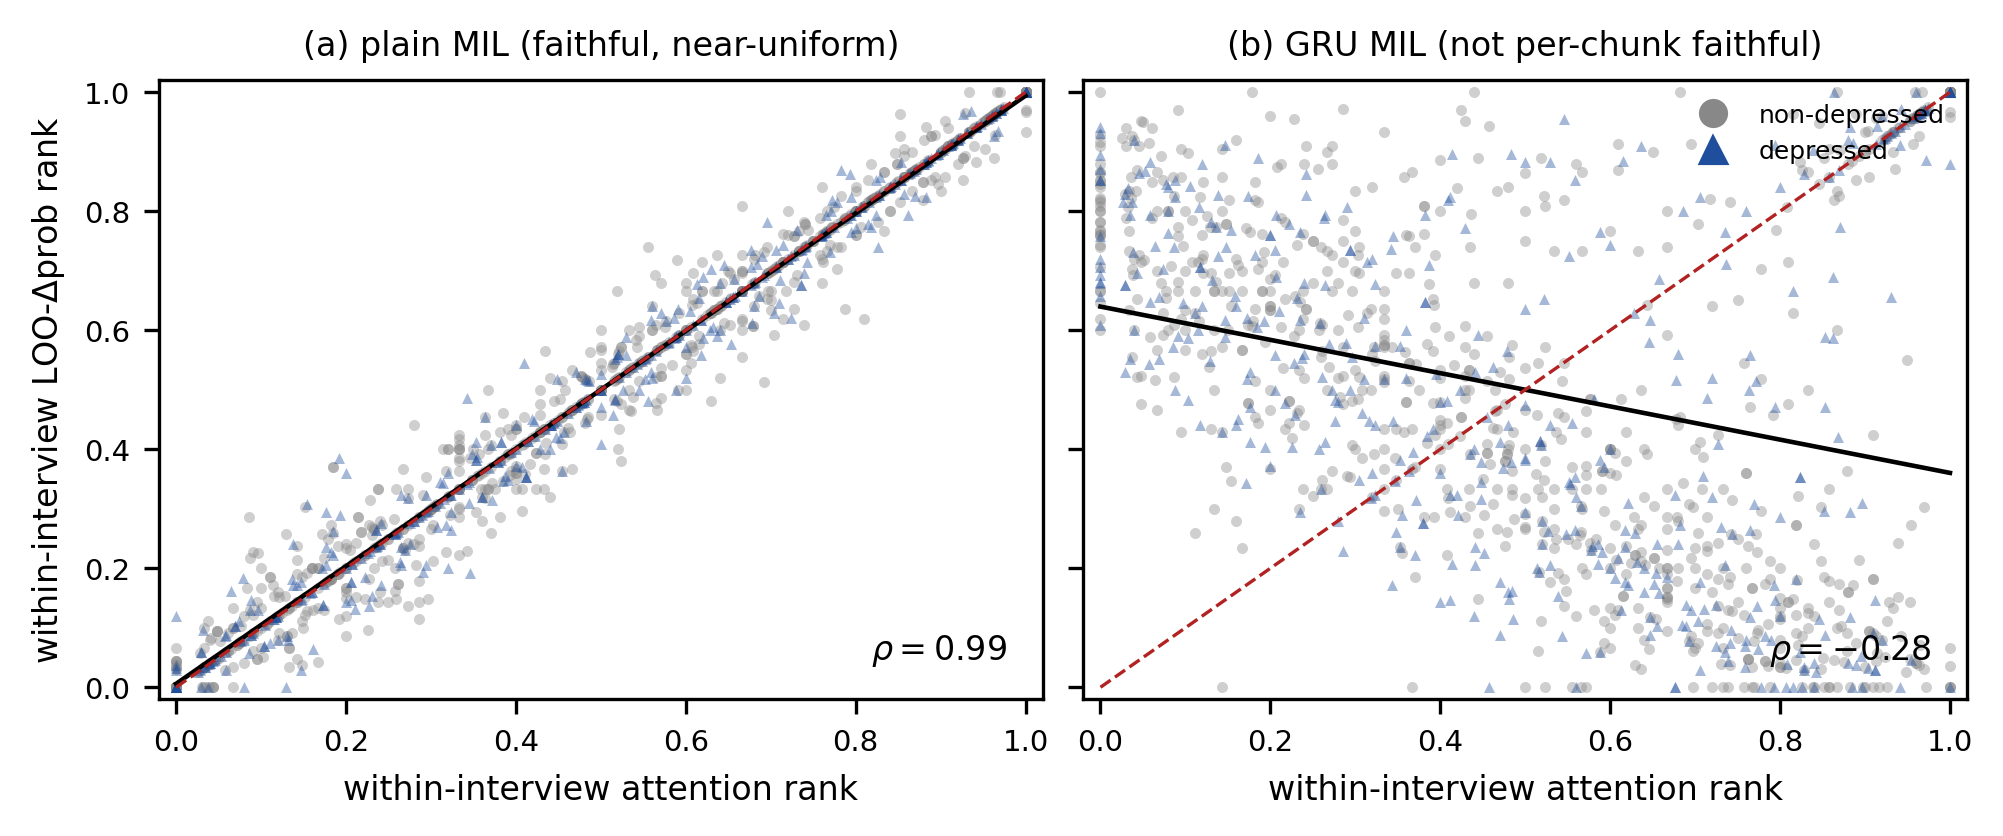
\includegraphics[width=\linewidth]{fig3_faithfulness.pdf}
      \\{\scriptsize Faithfulness is a property of the pooling, not of attention itself.}
    \end{column}
  \end{columns}
\end{frame}

\begin{frame}{What the model keys on --- a faithful explanation}
  \begin{center}
    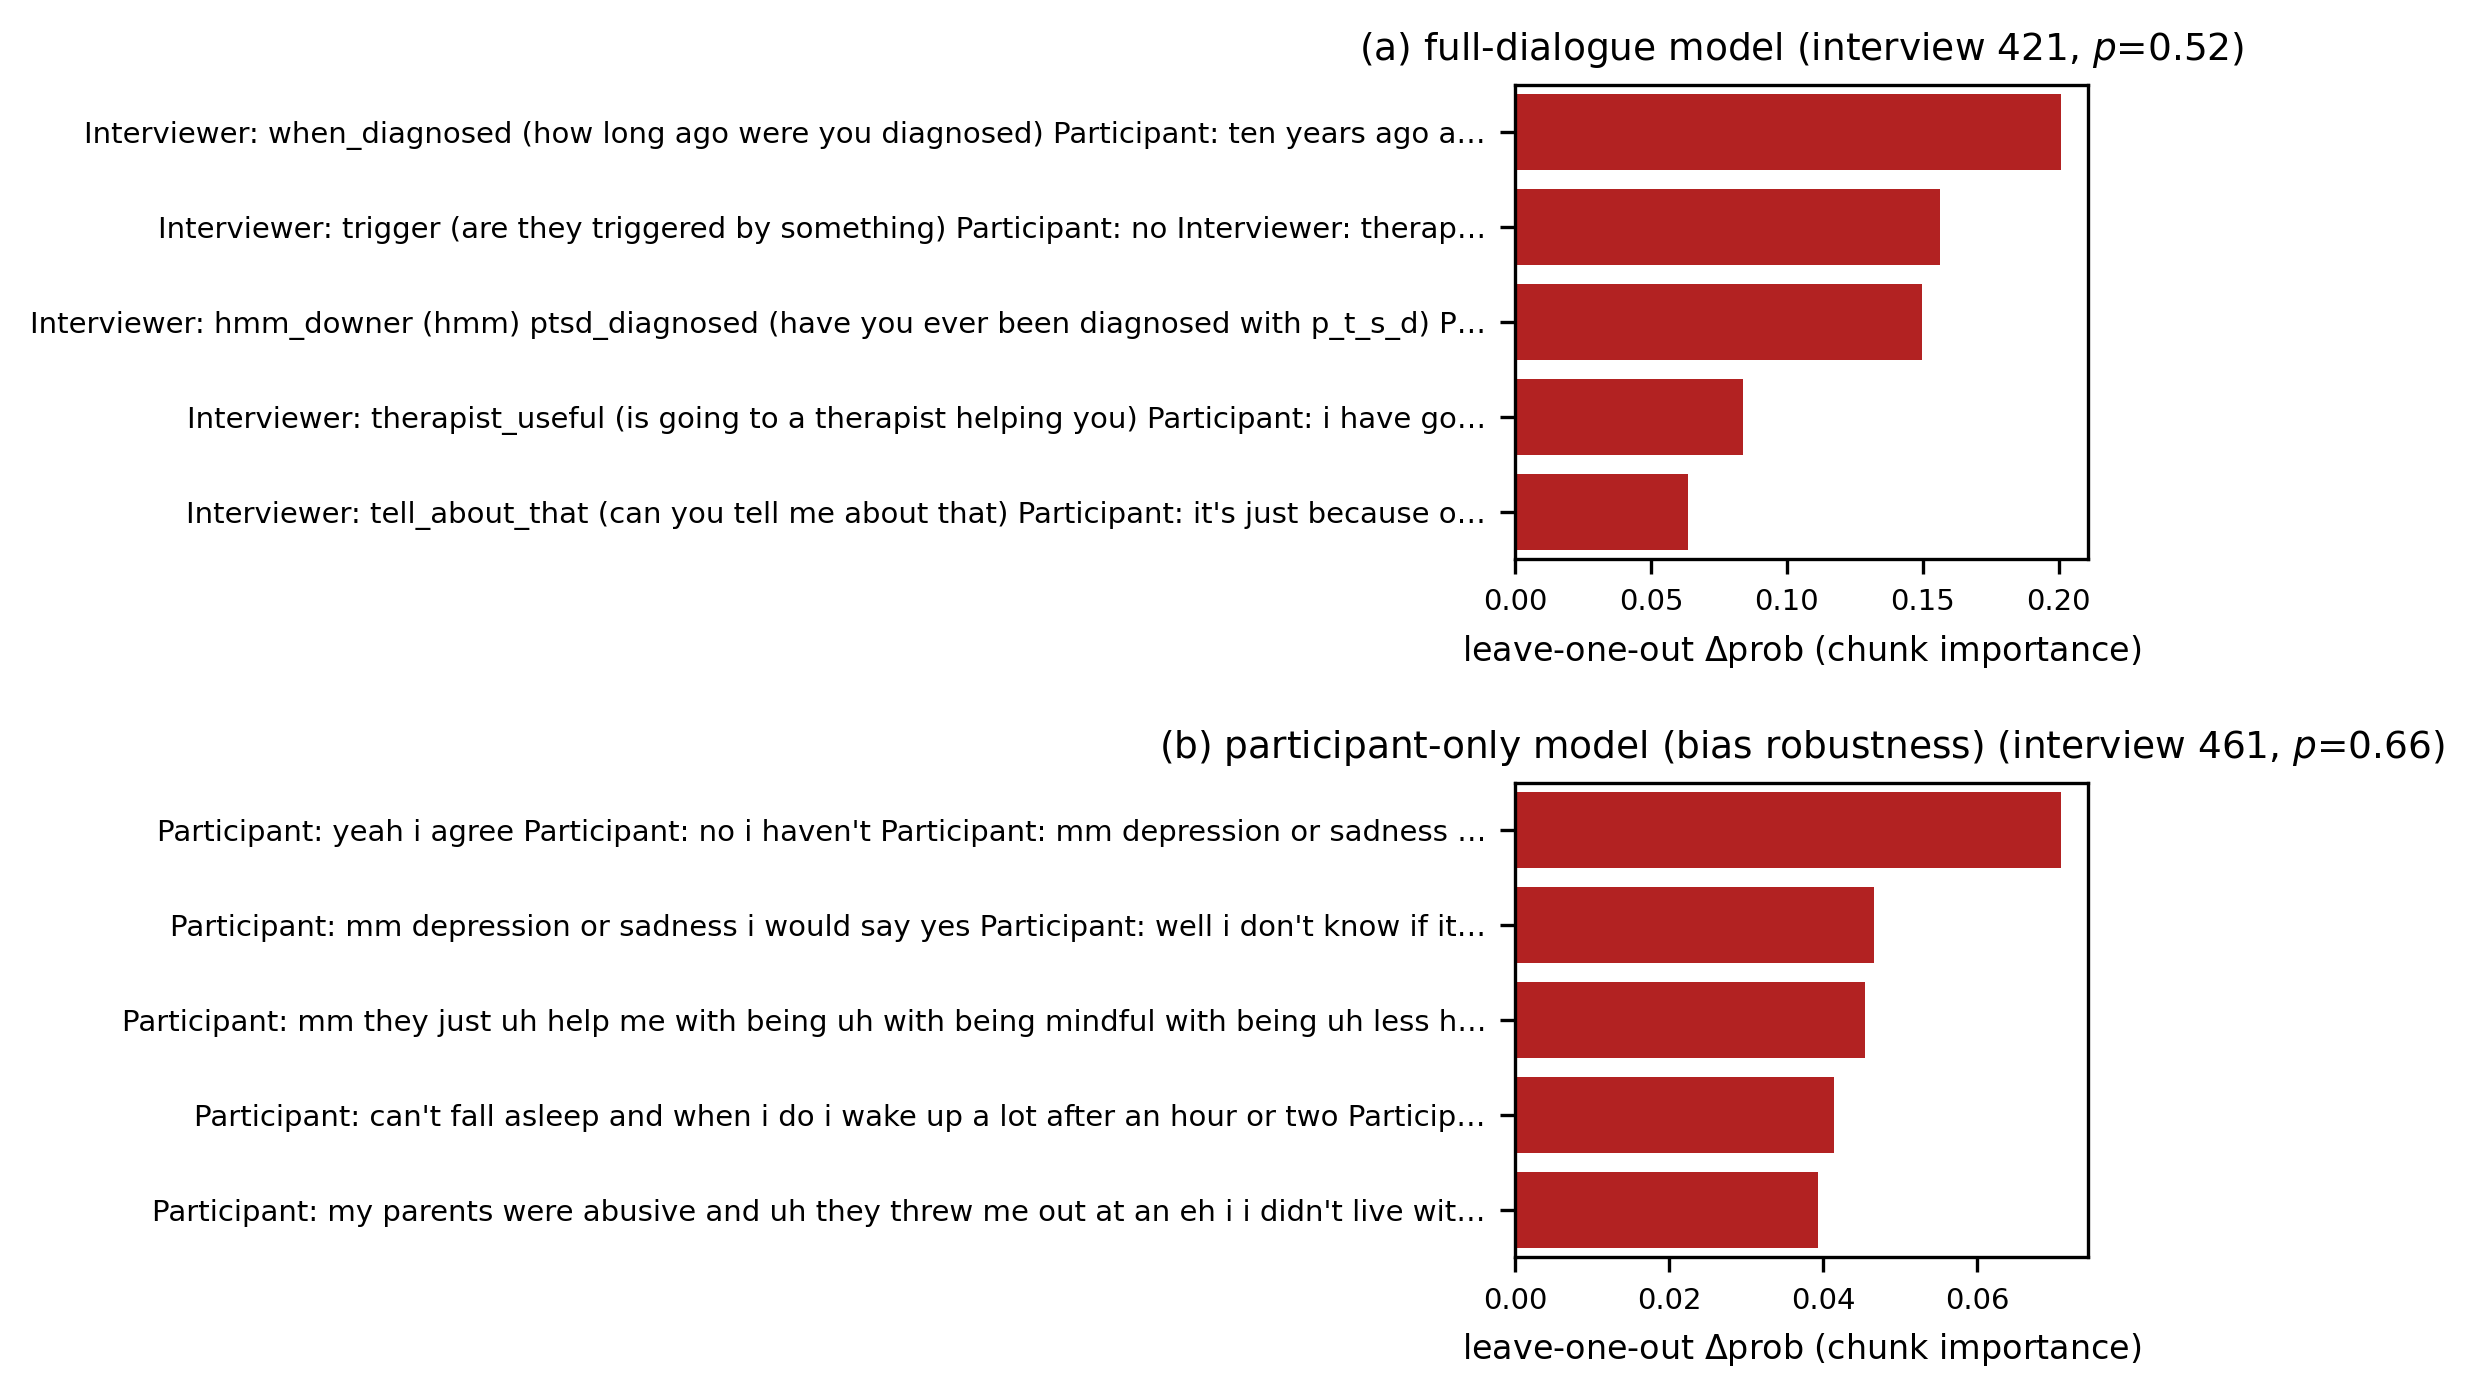
\includegraphics[width=0.6\textwidth]{fig_occlusion_attribution.pdf}
  \end{center}
  \begin{itemize}\small
    \item Top depression-supporting chunks (largest leave-one-out $\Delta$probability), by \emph{text}:
          \textbf{(a)} full dialogue $\to$ prior-diagnosis / therapy windows;
          \textbf{(b)} participant-only $\to$ own disclosures (low mood, sleep, trauma).
    \item Faithful, clinically sensible, \good{answer-driven} --- not a diagnostic-question shortcut.
  \end{itemize}
\end{frame}

\begin{frame}{No interviewer-prompt shortcut}
  \begin{itemize}
    \item The known shortcut: lean on the therapist's late mental-health questions.
    \item Our model's position--attention correlation is $\approx 0$
          (\num{+0.03} dev, \num{+0.002} test) --- attention is spread across the interview.
    \item Retrain with \emph{all interviewer lines removed} (participant-only):
          every metric \bad{drops} (AUC $0.868\!\rightarrow\!0.801$) \emph{and} the
          position--attention correlation \emph{rises} $+0.03\!\rightarrow\!+0.32$.
    \item[$\Rightarrow$] Stripped of context the model leans \emph{more} on position ---
          the opposite of one that had been riding the shortcut.
    \item[$\Rightarrow$] Prompts supply legitimate \emph{topical context}, not a removable shortcut.
  \end{itemize}
\end{frame}

\begin{frame}{Clinical read-out --- PHQ-8 symptom head}
  \begin{columns}[c]
    \begin{column}{0.58\textwidth}
      \centering
      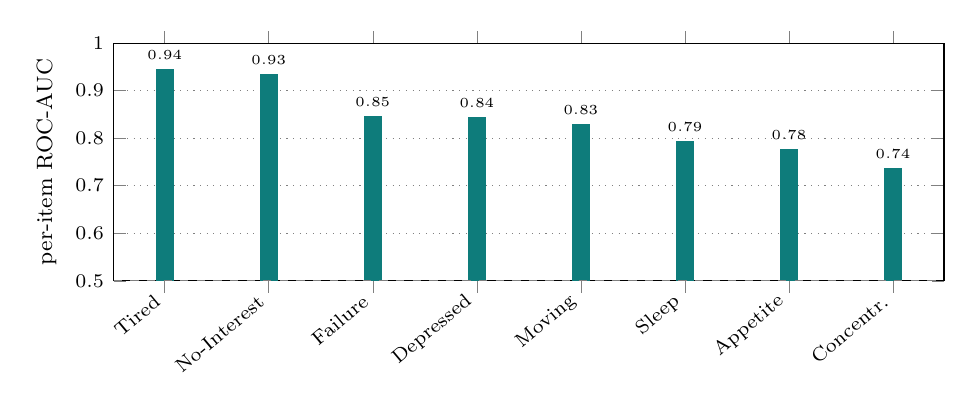
\begin{tikzpicture}
      \begin{axis}[
        ybar, width=\linewidth, height=4.6cm, bar width=6pt, ymin=0.5, ymax=1.0,
        ylabel={\footnotesize per-item ROC-AUC}, ylabel near ticks,
        symbolic x coords={Tired,No-Interest,Failure,Depressed,Moving,Sleep,Appetite,Concentr.},
        xtick=data, x tick label style={rotate=40,anchor=east,font=\scriptsize},
        ytick={0.5,0.6,0.7,0.8,0.9,1.0}, y tick label style={font=\scriptsize},
        ymajorgrids, grid style={dotted,gray},
        nodes near coords, nodes near coords style={font=\tiny},
        every node near coord/.append style={/pgf/number format/fixed,/pgf/number format/precision=2},
        enlarge x limits=0.07,
      ]
      \addplot[fill=mAccent,draw=mAccent] coordinates {
        (Tired,0.944) (No-Interest,0.934) (Failure,0.846) (Depressed,0.843)
        (Moving,0.829) (Sleep,0.793) (Appetite,0.776) (Concentr.,0.737)};
      \draw[dashed,gray] ({rel axis cs:0,0}|-{axis cs:Tired,0.5}) -- ({rel axis cs:1,0}|-{axis cs:Tired,0.5});
      \end{axis}
      \end{tikzpicture}
    \end{column}
    \begin{column}{0.42\textwidth}
      \begin{itemize}
        \item Auxiliary head predicts each PHQ-8 item; every symptom \good{above chance}
              (0.74--0.94 dev AUC).
        \item Strongest on the most lexicalised symptoms (fatigue, anhedonia), weakest on concentration.
        \item Attention concentrates on sleep / fatigue / mood chunks --- links the explanation
              to the diagnostic criteria.
      \end{itemize}
    \end{column}
  \end{columns}
\end{frame}

% --- fine-tuning slide commented out per request (re-enable: remove \iffalse/\fi) ---
\iffalse
\begin{frame}{Scientific honesty: fine-tuning does \emph{not} help}
  We asked whether fine-tuning the encoder lifts the ceiling. Pre-registered, staged search:
  \begin{itemize}
    \item Development grid showed a $\approx\!+0.02$ AUC ``lift'' (LoRA / last-$k$ / full).
    \item On a leakage-free OOF probe ($N{=}142$), the \good{frozen} encoder ranks \emph{first}.
    \item Cross-validation: the nominal gap \emph{flips sign} between schemes --- noise.
    \item No finalist beats the deployed frozen system; DAPT \bad{collapses} (catastrophic forgetting).
  \end{itemize}
  \begin{alertblock}{Why this is a strength}
    The staged protocol caught the development optimism \emph{before} the test split was spent ---
    we don't over-claim a win the data doesn't support.
  \end{alertblock}
\end{frame}
\fi

\begin{frame}{It generalises across corpora}
  \begin{columns}[c]
    \begin{column}{0.5\textwidth}
      \begin{itemize}\small
        \item Zero-shot transfer to E-DAIC (AVEC 2019): frozen model, no target adaptation, no threshold tuning.
        \item The model \good{transfers} --- and \emph{order-free} pooling transfers best
              (AUC \num{0.716}) over the temporal GRU (\num{0.662}).
        \item Lesson: the best \emph{in-domain} config is \bad{not} the best \emph{transfer}
              config --- generalisation-critical choices must be validated across corpora.
      \end{itemize}
    \end{column}
    \begin{column}{0.5\textwidth}
      \centering\footnotesize
      \setlength{\tabcolsep}{4pt}
      \begin{tabular}{@{}lcc@{}}
        \toprule
        & \multicolumn{2}{c}{\textbf{ROC-AUC}} \\
        \cmidrule(lr){2-3}
        \textbf{Source head} & \textbf{DAIC test} & \textbf{E-DAIC 0-shot} \\
        \midrule
        order-free (none) & \good{\num{.819}}{\tiny$\pm$.019}
          & \celld{\good{\num{.716}}}{.017}{.55,.88} \\[3pt]
        BiGRU & .786{\tiny$\pm$.040}
          & \celld{.662}{.011}{.48,.83} \\
        \bottomrule
      \end{tabular}
      \\[3pt]{\scriptsize 30-seed mean$\pm$std; E-DAIC adds subject-level
       bootstrap 95\% [CI] (56 test subjects). GRU wins DAIC \emph{dev} (.900), loses transfer.}
    \end{column}
  \end{columns}
\end{frame}

% =====================================================================
\section{Wrap-up}

\begin{frame}{Contributions \& takeaways}
  \textbf{Contributions}
  \begin{enumerate}
    \item \textbf{TC-MIL} --- dialogue-chunk instances turn degenerate turns into discriminative ones.
    \item \textbf{A leakage-free protocol} under which a single network beats the cleanest verified
          baseline and matches the best reported single model.
    \item \textbf{Extensive validation} --- ablations, internal cross-validation, measured
          interpretability, and an explicit bias control.
  \end{enumerate}
  \vfill
  \textbf{Takeaways}
  \begin{itemize}
    \item \good{The instance definition}, not the aggregation network, carries the signal.
    \item \good{Honest evaluation is a feature}: the protocol makes the numbers trustworthy and comparable.
    \item \good{Trust is measured}: faithfulness quantified, the interviewer-prompt shortcut ruled out.
  \end{itemize}
  \vfill
  \begin{center}\small Code \& weights: \href{https://github.com/SaverioNapolitano/tcmil}{\texttt{github.com/SaverioNapolitano/tcmil}}\end{center}
\end{frame}

\begin{frame}[standout]
  Thank you --- questions?
\end{frame}

% =====================================================================
\appendix
\backupbegin
\section{Backup: full tables}

\begin{frame}{Backup --- architecture ladder (official split, all metrics)}
  \begin{center}\scriptsize
  \resizebox{\textwidth}{!}{%
  \begin{tabular}{@{}lcccccccc@{}}
    \toprule
    \textbf{Architecture} & \textbf{UAR} & \textbf{Prec.} & \textbf{Recall} & \textbf{pos-F1} & \textbf{macro-F1} & \textbf{micro-F1} & \textbf{PR-AUC} & \textbf{ROC-AUC} \\
    \midrule
    dialogue mean & \celld{.56}{.06}{.45,.76} & \celld{.27}{.26}{.00,.58} & \celld{.26}{.26}{.00,.86} & \celld{.24}{.23}{.00,.67} & \celld{.51}{.10}{.38,.71} & \celld{.68}{.04}{.47,.77} & \celld{.50}{.07}{.27,.73} & \celld{.66}{.04}{.47,.82} \\
    flat MIL, mean & \celld{.51}{.02}{.50,.50} & \celld{.11}{.18}{.00,.00} & \celld{.08}{.14}{.00,.00} & \celld{.09}{.14}{.00,.00} & \celld{.45}{.05}{.36,.47} & \celld{.68}{.04}{.55,.83} & \celld{.40}{.09}{.22,.63} & \celld{.61}{.08}{.42,.75} \\
    flat MIL, attn & \celld{.53}{.04}{.45,.77} & \celld{.22}{.25}{.19,.73} & \celld{.18}{.20}{.18,.71} & \celld{.18}{.19}{.19,.67} & \celld{.48}{.08}{.45,.76} & \celld{.67}{.04}{.53,.81} & \celld{.48}{.10}{.31,.78} & \celld{.67}{.09}{.57,.86} \\
    DAMIL-R & \celld{.66}{.06}{.53,.85} & \celld{.55}{.09}{.29,.85} & \celld{.50}{.12}{.31,.80} & \celld{.51}{.10}{.31,.77} & \celld{.66}{.06}{.53,.84} & \celld{.73}{.05}{.62,.87} & \celld{.59}{.08}{.38,.84} & \celld{.75}{.06}{.64,.90} \\
    SS-DAMIL-R (MH) & \celld{.67}{.06}{.51,.85} & \celld{.58}{.11}{.29,.85} & \celld{.51}{.13}{.29,.80} & \celld{.53}{.12}{.30,.77} & \celld{.67}{.07}{.51,.84} & \celld{.74}{.03}{.60,.87} & \celld{.60}{.08}{.39,.84} & \celld{.76}{.05}{.62,.91} \\
    SS-DAMIL-R (GSI) & \celld{.66}{.06}{.53,.84} & \celld{.53}{.09}{.31,.83} & \celld{.50}{.12}{.31,.80} & \celld{.51}{.11}{.32,.75} & \celld{.66}{.07}{.53,.83} & \celld{.72}{.05}{.60,.85} & \celld{.57}{.10}{.41,.85} & \celld{.75}{.07}{.64,.91} \\
    SS-DAMIL-R (Conv) & \celld{.65}{.06}{.51,.83} & \celld{.53}{.09}{.29,.83} & \celld{.50}{.07}{.29,.78} & \celld{.51}{.07}{.30,.74} & \celld{.65}{.07}{.51,.82} & \celld{.71}{.07}{.60,.85} & \celld{.61}{.09}{.42,.86} & \celld{.75}{.08}{.65,.91} \\
    \midrule
    \textbf{TC-MIL} & \celld{\textbf{.77}}{.03}{.59,.92} & \celld{\textbf{.70}}{.04}{.36,.93} & \celld{\textbf{.66}}{.04}{.40,.91} & \celld{\textbf{.68}}{.04}{.41,.86} & \celld{\textbf{.77}}{.03}{.59,.90} & \celld{\textbf{.81}}{.02}{.66,.91} & \celld{\textbf{.62}}{.02}{.42,.93} & \celld{\textbf{.86}}{.01}{.75,.96} \\
    \bottomrule
  \end{tabular}}
  \end{center}
  {\scriptsize 30-seed per-seed mean$\pm$std (top) and subject-level bootstrap 95\% CI (bottom, 2000 resamples).}
\end{frame}

\begin{frame}{Backup --- single-lever study (official split)}
  \begin{center}\small
  \begin{tabular}{@{}llccc@{}}
    \toprule
    \textbf{Lever} & \textbf{Change} & \textbf{mac-F1} & \textbf{mic-F1} & \textbf{AUC} \\
    \midrule
    0 & baseline ($pos\_weight\!\approx\!2.5$) & 0.751{\footnotesize$\pm$.032} & 0.794{\footnotesize$\pm$.026} & 0.856{\footnotesize$\pm$.011} \\
    1 & OOF threshold & 0.750{\footnotesize$\pm$.028} & 0.773{\footnotesize$\pm$.025} & 0.864{\footnotesize$\pm$.011} \\
    2 & temperature scaling & no gain & no gain & 0.856$^{\dagger}$ \\
    \textbf{3} & \textbf{$pos\_weight\!=\!1.0$} & \textbf{0.774}{\footnotesize$\pm$.029} & \textbf{0.814}{\footnotesize$\pm$.024} & \textbf{0.864}{\footnotesize$\pm$.011} \\
    4 & symptom decision & no gain & no gain & 0.856$^{\dagger}$ \\
    5 & richer encoder (1.5B) & 0.695{\footnotesize$\pm$.060} & 0.753{\footnotesize$\pm$.036} & 0.804{\footnotesize$\pm$.050} \\
    6 & MC-dropout (T=30) & 0.771{\footnotesize$\pm$.036} & 0.812{\footnotesize$\pm$.029} & 0.864{\footnotesize$\pm$.012} \\
    7 & multi-granularity bags & 0.782{\footnotesize$\pm$.070} & 0.825{\footnotesize$\pm$.040} & 0.867{\footnotesize$\pm$.010} \\
    8 & dev-prevalence threshold & 0.773{\footnotesize$\pm$.021} & 0.802{\footnotesize$\pm$.018} & 0.864{\footnotesize$\pm$.011} \\
    \bottomrule
  \end{tabular}
  \end{center}
  {\scriptsize Only the class weight (lever 3) transfers robustly. $^{\dagger}$calibration/decision deltas, no per-seed probabilities; AUC unchanged.}
\end{frame}

\begin{frame}{Backup --- design ablation I (representation, dev, 5 seeds)}
  \begin{columns}[T]
  \begin{column}{0.5\textwidth}\scriptsize
  \textit{Encoder (GRU, $w4/s2$)}
  \begin{tabular}{@{}lccc@{}}
    \toprule
    \textbf{Variant} & \textbf{AUC} & \textbf{mac-F1} & \textbf{pos-F1} \\
    \midrule
    \textbf{bge-large (base)} & \textbf{.909}{\tiny$\pm$.005} & \textbf{.792}{\tiny$\pm$.034} & \textbf{.714}{\tiny$\pm$.059} \\
    UAE-large & .915{\tiny$\pm$.003} & .796{\tiny$\pm$.035} & .724{\tiny$\pm$.060} \\
    mxbai-large & .912{\tiny$\pm$.007} & .772{\tiny$\pm$.038} & .685{\tiny$\pm$.068} \\
    bge-base & .913{\tiny$\pm$.003} & .772{\tiny$\pm$.073} & .673{\tiny$\pm$.120} \\
    all-mpnet & .890{\tiny$\pm$.009} & .789{\tiny$\pm$.033} & .713{\tiny$\pm$.046} \\
    gte-large & .891{\tiny$\pm$.013} & .743{\tiny$\pm$.048} & .643{\tiny$\pm$.085} \\
    e5-large & .897{\tiny$\pm$.012} & .709{\tiny$\pm$.090} & .587{\tiny$\pm$.167} \\
    \bottomrule
  \end{tabular}
  \end{column}
  \begin{column}{0.5\textwidth}\scriptsize
  \textit{Temporal head (bge-large, $w4/s2$)}
  \begin{tabular}{@{}lccc@{}}
    \toprule
    \textbf{Variant} & \textbf{AUC} & \textbf{mac-F1} & \textbf{pos-F1} \\
    \midrule
    \textbf{none (plain)} & \textbf{.876}{\tiny$\pm$.001} & \textbf{.645}{\tiny$\pm$.100} & \textbf{.473}{\tiny$\pm$.180} \\
    GRU (base) & .909{\tiny$\pm$.005} & .792{\tiny$\pm$.034} & .714{\tiny$\pm$.059} \\
    GRU 2-layer & .912{\tiny$\pm$.009} & .794{\tiny$\pm$.023} & .746{\tiny$\pm$.029} \\
    Transformer & .917{\tiny$\pm$.012} & .779{\tiny$\pm$.058} & .722{\tiny$\pm$.065} \\
    \bottomrule
  \end{tabular}
  \vspace{2mm}
  {\tiny Plain head fixed a priori for faithful linear attribution, not the dev argmax.}
  \end{column}
  \end{columns}
\end{frame}

\begin{frame}{Backup --- design ablation II (granularity / regularisation, dev)}
  \begin{center}\small
  \begin{tabular}{@{}lccc@{}}
    \toprule
    \textbf{Variant} & \textbf{dev AUC} & \textbf{dev mac-F1} & \textbf{dev pos-F1} \\
    \midrule
    \multicolumn{4}{@{}l}{\emph{Window / stride}} \\
    $w2/s1$ & .915{\footnotesize$\pm$.004} & .733{\footnotesize$\pm$.081} & .605{\footnotesize$\pm$.134} \\
    \textbf{$w4/s2$ (base)} & \textbf{.909}{\footnotesize$\pm$.005} & \textbf{.792}{\footnotesize$\pm$.034} & \textbf{.714}{\footnotesize$\pm$.059} \\
    $w6/s3$ & .919{\footnotesize$\pm$.010} & .793{\footnotesize$\pm$.076} & .708{\footnotesize$\pm$.125} \\
    $w4/s1$ & .899{\footnotesize$\pm$.007} & .750{\footnotesize$\pm$.036} & .637{\footnotesize$\pm$.057} \\
    \midrule
    \multicolumn{4}{@{}l}{\emph{Regularisation / capacity}} \\
    dropout 0.3 & .911{\footnotesize$\pm$.004} & .813{\footnotesize$\pm$.024} & .752{\footnotesize$\pm$.033} \\
    \textbf{dropout 0.4 (base)} & \textbf{.909}{\footnotesize$\pm$.005} & \textbf{.792}{\footnotesize$\pm$.034} & \textbf{.714}{\footnotesize$\pm$.059} \\
    dropout 0.5 & .912{\footnotesize$\pm$.005} & .799{\footnotesize$\pm$.038} & .722{\footnotesize$\pm$.063} \\
    proj-dim 192 & .909{\footnotesize$\pm$.006} & .785{\footnotesize$\pm$.020} & .714{\footnotesize$\pm$.035} \\
    aux-weight 0.0 & .909{\footnotesize$\pm$.005} & .824{\footnotesize$\pm$.017} & .763{\footnotesize$\pm$.029} \\
    aux-weight 0.15 & .908{\footnotesize$\pm$.004} & .797{\footnotesize$\pm$.042} & .718{\footnotesize$\pm$.074} \\
    aux-weight 0.5 & .914{\footnotesize$\pm$.005} & .797{\footnotesize$\pm$.034} & .725{\footnotesize$\pm$.057} \\
    \bottomrule
  \end{tabular}
  \end{center}
\end{frame}

\begin{frame}{Backup --- internal cross-validation, $K$-Fold}
  \begin{center}\scriptsize
  \resizebox{\textwidth}{!}{%
  \begin{tabular}{@{}llcccccccc@{}}
    \toprule
    \textbf{Proto} & \textbf{Model} & \textbf{UAR} & \textbf{Prec.} & \textbf{Recall} & \textbf{pos-F1} & \textbf{macro-F1} & \textbf{micro-F1} & \textbf{PR-AUC} & \textbf{ROC-AUC} \\
    \midrule
    \multirow{8}{*}{$K$-Fold}
     & dialogue mean & \celld{.55}{.08}{.51,.59} & \celld{.23}{.29}{.10,.40} & \celld{.22}{.31}{.08,.39} & \celld{.19}{.23}{.08,.32} & \celld{.49}{.10}{.44,.54} & \celld{.68}{.05}{.66,.70} & \celld{.58}{.13}{.51,.64} & \celld{.73}{.07}{.69,.76} \\
     & flat MIL, mean & \celld{.52}{.06}{.50,.56} & \celld{.11}{.23}{.00,.24} & \celld{.08}{.17}{.00,.17} & \celld{.09}{.19}{.00,.19} & \celld{.46}{.10}{.41,.51} & \celld{.71}{.04}{.69,.73} & \celld{.52}{.08}{.48,.56} & \celld{.69}{.08}{.65,.73} \\
     & flat MIL, attn & \celld{.52}{.04}{.50,.55} & \celld{.10}{.22}{.00,.23} & \celld{.07}{.14}{.00,.15} & \celld{.08}{.17}{.00,.17} & \celld{.45}{.08}{.41,.50} & \celld{.70}{.03}{.69,.72} & \celld{.51}{.10}{.46,.56} & \celld{.66}{.11}{.61,.71} \\
     & DAMIL-R & \celld{.68}{.13}{.62,.74} & \celld{.55}{.17}{.46,.63} & \celld{.55}{.19}{.45,.64} & \celld{.55}{.18}{.46,.63} & \celld{.68}{.13}{.61,.74} & \celld{.73}{.10}{.68,.78} & \celld{.62}{.15}{.54,.69} & \celld{.75}{.13}{.68,.81} \\
     & SS-DAMIL-R (MH) & \celld{.64}{.11}{.58,.70} & \celld{.50}{.16}{.41,.57} & \celld{.51}{.18}{.41,.60} & \celld{.49}{.16}{.41,.57} & \celld{.64}{.11}{.58,.69} & \celld{.70}{.10}{.65,.74} & \celld{.59}{.15}{.51,.66} & \celld{.71}{.12}{.65,.77} \\
     & SS-DAMIL-R (GSI) & \celld{.66}{.10}{.61,.71} & \celld{.51}{.12}{.45,.57} & \celld{.54}{.13}{.48,.61} & \celld{.52}{.12}{.46,.58} & \celld{.65}{.10}{.61,.70} & \celld{.71}{.09}{.66,.75} & \celld{.60}{.10}{.55,.65} & \celld{.76}{.08}{.72,.80} \\
     & SS-DAMIL-R (Conv) & \celld{.62}{.10}{.57,.67} & \celld{.46}{.22}{.34,.57} & \celld{.42}{.23}{.30,.54} & \celld{.42}{.21}{.31,.52} & \celld{.61}{.12}{.55,.67} & \celld{.71}{.08}{.66,.74} & \celld{.58}{.15}{.51,.66} & \celld{.71}{.11}{.65,.76} \\
     & \textbf{TC-MIL} & \celld{\textbf{.70}}{.11}{.69,.72} & \celld{\textbf{.59}}{.20}{.56,.63} & \celld{\textbf{.55}}{.21}{.52,.59} & \celld{\textbf{.56}}{.20}{.53,.60} & \celld{\textbf{.70}}{.12}{.68,.72} & \celld{\textbf{.77}}{.08}{.75,.78} & \celld{\textbf{.67}}{.13}{.65,.70} & \celld{\textbf{.79}}{.09}{.78,.81} \\
    \bottomrule
  \end{tabular}}
  \end{center}
  {\scriptsize Per-run mean$\pm$std (top) and 95\% CI of the mean (bottom). TC-MIL leads every column.}
\end{frame}

\begin{frame}{Backup --- internal cross-validation, Monte-Carlo}
  \begin{center}\scriptsize
  \resizebox{\textwidth}{!}{%
  \begin{tabular}{@{}llcccccccc@{}}
    \toprule
    \textbf{Proto} & \textbf{Model} & \textbf{UAR} & \textbf{Prec.} & \textbf{Recall} & \textbf{pos-F1} & \textbf{macro-F1} & \textbf{micro-F1} & \textbf{PR-AUC} & \textbf{ROC-AUC} \\
    \midrule
    \multirow{8}{*}{MC}
     & dialogue mean & \celld{.53}{.05}{.51,.56} & \celld{.12}{.20}{.03,.23} & \celld{.13}{.24}{.02,.27} & \celld{.12}{.20}{.03,.23} & \celld{.46}{.08}{.42,.50} & \celld{.68}{.04}{.65,.69} & \celld{.57}{.12}{.51,.64} & \celld{.70}{.09}{.66,.75} \\
     & flat MIL, mean & \celld{.51}{.02}{.50,.52} & \celld{.08}{.16}{.00,.17} & \celld{.10}{.23}{.00,.22} & \celld{.07}{.16}{.00,.16} & \celld{.43}{.04}{.41,.45} & \celld{.66}{.06}{.63,.69} & \celld{.57}{.12}{.51,.63} & \celld{.69}{.13}{.61,.75} \\
     & flat MIL, attn & \celld{.55}{.05}{.52,.58} & \celld{.42}{.38}{.23,.62} & \celld{.14}{.17}{.06,.23} & \celld{.18}{.18}{.10,.28} & \celld{.50}{.09}{.46,.55} & \celld{.70}{.02}{.70,.71} & \celld{.57}{.09}{.52,.61} & \celld{.71}{.08}{.67,.75} \\
     & DAMIL-R & \celld{.66}{.15}{.59,.73} & \celld{.52}{.22}{.41,.64} & \celld{.50}{.25}{.38,.62} & \celld{.51}{.23}{.39,.62} & \celld{.65}{.15}{.58,.73} & \celld{.72}{.11}{.66,.77} & \celld{.57}{.18}{.48,.66} & \celld{.73}{.13}{.67,.80} \\
     & SS-DAMIL-R (MH) & \celld{.68}{.12}{.62,.74} & \celld{.55}{.17}{.47,.64} & \celld{.59}{.17}{.50,.67} & \celld{.56}{.16}{.48,.64} & \celld{.68}{.12}{.61,.74} & \celld{.72}{.11}{.66,.77} & \celld{.62}{.15}{.54,.69} & \celld{.75}{.13}{.68,.81} \\
     & SS-DAMIL-R (GSI) & \celld{.66}{.11}{.60,.72} & \celld{.54}{.16}{.46,.62} & \celld{.53}{.15}{.44,.61} & \celld{.53}{.15}{.45,.60} & \celld{.66}{.11}{.60,.72} & \celld{.71}{.10}{.66,.76} & \celld{.57}{.14}{.50,.65} & \celld{.72}{.13}{.65,.78} \\
     & SS-DAMIL-R (Conv) & \celld{.63}{.07}{.60,.67} & \celld{.48}{.20}{.37,.57} & \celld{.43}{.20}{.33,.52} & \celld{.45}{.19}{.34,.54} & \celld{.62}{.10}{.57,.67} & \celld{.71}{.04}{.69,.73} & \celld{.63}{.11}{.57,.68} & \celld{.76}{.09}{.72,.81} \\
     & \textbf{TC-MIL} & \celld{\textbf{.73}}{.09}{.70,.75} & \celld{\textbf{.63}}{.20}{.57,.68} & \celld{\textbf{.59}}{.21}{.53,.65} & \celld{\textbf{.60}}{.20}{.54,.65} & \celld{\textbf{.72}}{.11}{.69,.75} & \celld{\textbf{.78}}{.07}{.76,.79} & \celld{\textbf{.71}}{.09}{.68,.74} & \celld{\textbf{.82}}{.05}{.81,.84} \\
    \bottomrule
  \end{tabular}}
  \end{center}
  {\scriptsize Per-run mean$\pm$std (top) and 95\% CI of the mean (bottom). TC-MIL leads every column of both protocols.}
\end{frame}

\begin{frame}[shrink=50]{Backup --- significance, official split (30 per-seed scores)}
  \begin{columns}[T]
  \begin{column}{0.5\textwidth}\centering\small
  \begin{tabular}{@{}llcc@{}}
    \toprule
    \textbf{Comparison} & \textbf{Metric} & \textbf{Welch's $t$} & \textbf{Mann--Whitney $U$} \\
    \midrule
    \multirow{8}{*}{vs dialogue mean} & UAR & $<$.001$^{*}$ & $<$.001$^{*}$ \\
     & Precision & $<$.001$^{*}$ & $<$.001$^{*}$ \\ & Recall & $<$.001$^{*}$ & $<$.001$^{*}$ \\
     & pos-F1 & $<$.001$^{*}$ & $<$.001$^{*}$ \\ & macro-F1 & $<$.001$^{*}$ & $<$.001$^{*}$ \\
     & micro-F1 & $<$.001$^{*}$ & $<$.001$^{*}$ \\ & PR-AUC & $<$.001$^{*}$ & $<$.001$^{*}$ \\ & ROC-AUC & $<$.001$^{*}$ & $<$.001$^{*}$ \\
    \midrule
    \multirow{8}{*}{vs flat MIL, mean} & UAR & $<$.001$^{*}$ & $<$.001$^{*}$ \\
     & Precision & $<$.001$^{*}$ & $<$.001$^{*}$ \\ & Recall & $<$.001$^{*}$ & $<$.001$^{*}$ \\
     & pos-F1 & $<$.001$^{*}$ & $<$.001$^{*}$ \\ & macro-F1 & $<$.001$^{*}$ & $<$.001$^{*}$ \\
     & micro-F1 & $<$.001$^{*}$ & $<$.001$^{*}$ \\ & PR-AUC & $<$.001$^{*}$ & $<$.001$^{*}$ \\ & ROC-AUC & $<$.001$^{*}$ & $<$.001$^{*}$ \\
    \midrule
    \multirow{8}{*}{vs flat MIL, attn} & UAR & $<$.001$^{*}$ & $<$.001$^{*}$ \\
     & Precision & $<$.001$^{*}$ & $<$.001$^{*}$ \\ & Recall & $<$.001$^{*}$ & $<$.001$^{*}$ \\
     & pos-F1 & $<$.001$^{*}$ & $<$.001$^{*}$ \\ & macro-F1 & $<$.001$^{*}$ & $<$.001$^{*}$ \\
     & micro-F1 & $<$.001$^{*}$ & $<$.001$^{*}$ \\ & PR-AUC & $<$.001$^{*}$ & $<$.001$^{*}$ \\ & ROC-AUC & $<$.001$^{*}$ & $<$.001$^{*}$ \\
    \midrule
    \multirow{8}{*}{vs DAMIL-R} & UAR & $<$.001$^{*}$ & $<$.001$^{*}$ \\
     & Precision & $<$.001$^{*}$ & $<$.001$^{*}$ \\ & Recall & $<$.001$^{*}$ & $<$.001$^{*}$ \\
     & pos-F1 & $<$.001$^{*}$ & $<$.001$^{*}$ \\ & macro-F1 & $<$.001$^{*}$ & $<$.001$^{*}$ \\
     & micro-F1 & $<$.001$^{*}$ & $<$.001$^{*}$ \\ & PR-AUC & 0.055 & 0.176 \\ & ROC-AUC & $<$.001$^{*}$ & $<$.001$^{*}$ \\
    \bottomrule
  \end{tabular}
  \end{column}
  \begin{column}{0.5\textwidth}\centering\small
  \begin{tabular}{@{}llcc@{}}
    \toprule
    \textbf{Comparison} & \textbf{Metric} & \textbf{Welch's $t$} & \textbf{Mann--Whitney $U$} \\
    \midrule
    \multirow{8}{*}{vs SS-DAMIL-R (MH)} & UAR & $<$.001$^{*}$ & $<$.001$^{*}$ \\
     & Precision & $<$.001$^{*}$ & $<$.001$^{*}$ \\ & Recall & $<$.001$^{*}$ & $<$.001$^{*}$ \\
     & pos-F1 & $<$.001$^{*}$ & $<$.001$^{*}$ \\ & macro-F1 & $<$.001$^{*}$ & $<$.001$^{*}$ \\
     & micro-F1 & $<$.001$^{*}$ & $<$.001$^{*}$ \\ & PR-AUC & 0.397 & 0.311 \\ & ROC-AUC & $<$.001$^{*}$ & $<$.001$^{*}$ \\
    \midrule
    \multirow{8}{*}{vs SS-DAMIL-R (GSI)} & UAR & $<$.001$^{*}$ & $<$.001$^{*}$ \\
     & Precision & $<$.001$^{*}$ & $<$.001$^{*}$ \\ & Recall & $<$.001$^{*}$ & $<$.001$^{*}$ \\
     & pos-F1 & $<$.001$^{*}$ & $<$.001$^{*}$ \\ & macro-F1 & $<$.001$^{*}$ & $<$.001$^{*}$ \\
     & micro-F1 & $<$.001$^{*}$ & $<$.001$^{*}$ \\ & PR-AUC & 0.010$^{*}$ & 0.027$^{*}$ \\ & ROC-AUC & $<$.001$^{*}$ & $<$.001$^{*}$ \\
    \midrule
    \multirow{8}{*}{vs SS-DAMIL-R (Conv)} & UAR & $<$.001$^{*}$ & $<$.001$^{*}$ \\
     & Precision & $<$.001$^{*}$ & $<$.001$^{*}$ \\ & Recall & $<$.001$^{*}$ & $<$.001$^{*}$ \\
     & pos-F1 & $<$.001$^{*}$ & $<$.001$^{*}$ \\ & macro-F1 & $<$.001$^{*}$ & $<$.001$^{*}$ \\
     & micro-F1 & $<$.001$^{*}$ & $<$.001$^{*}$ \\ & PR-AUC & 0.527 & 0.751 \\ & ROC-AUC & $<$.001$^{*}$ & $<$.001$^{*}$ \\
    \bottomrule
  \end{tabular}
  \end{column}
  \end{columns}
  \vfill
  {\scriptsize $^{*}p<0.05$. One-sample $t$ of 30 per-seed macro-F1 vs Milintsevich 0.739: $p=3.8\times10^{-7}$.}
\end{frame}

\begin{frame}[shrink=50]{Backup --- significance, internal CV (paired, $n{=}15$ runs)}
  \begin{columns}[T]
  \begin{column}{0.5\textwidth}\centering\small
  \begin{tabular}{@{}llcccc@{}}
    \toprule
    & & \multicolumn{2}{c}{\textbf{Monte Carlo}} & \multicolumn{2}{c}{\textbf{$K$-Fold}} \\
    \cmidrule(lr){3-4}\cmidrule(lr){5-6}
    \textbf{Comparison} & \textbf{Metric} & \textbf{Wilcoxon} & \textbf{paired $t$} & \textbf{Wilcoxon} & \textbf{paired $t$} \\
    \midrule
    \multirow{8}{*}{vs dialogue mean}
     & UAR & $<$.001$^{*}$ & $<$.001$^{*}$ & 0.007$^{*}$ & 0.003$^{*}$ \\
     & Precision & $<$.001$^{*}$ & $<$.001$^{*}$ & 0.014$^{*}$ & 0.009$^{*}$ \\
     & Recall & $<$.001$^{*}$ & $<$.001$^{*}$ & 0.023$^{*}$ & 0.015$^{*}$ \\
     & pos-F1 & $<$.001$^{*}$ & $<$.001$^{*}$ & 0.005$^{*}$ & 0.002$^{*}$ \\
     & macro-F1 & $<$.001$^{*}$ & $<$.001$^{*}$ & 0.004$^{*}$ & $<$.001$^{*}$ \\
     & micro-F1 & $<$.001$^{*}$ & $<$.001$^{*}$ & 0.008$^{*}$ & 0.004$^{*}$ \\
     & PR-AUC & $<$.001$^{*}$ & $<$.001$^{*}$ & 0.055 & 0.060 \\
     & ROC-AUC & 0.005$^{*}$ & 0.002$^{*}$ & 0.084 & 0.191 \\
    \midrule
    \multirow{8}{*}{vs flat MIL, mean}
     & UAR & $<$.001$^{*}$ & $<$.001$^{*}$ & 0.008$^{*}$ & 0.004$^{*}$ \\
     & Precision & $<$.001$^{*}$ & $<$.001$^{*}$ & 0.015$^{*}$ & 0.002$^{*}$ \\
     & Recall & 0.001$^{*}$ & $<$.001$^{*}$ & 0.005$^{*}$ & 0.001$^{*}$ \\
     & pos-F1 & $<$.001$^{*}$ & $<$.001$^{*}$ & 0.006$^{*}$ & 0.002$^{*}$ \\
     & macro-F1 & $<$.001$^{*}$ & $<$.001$^{*}$ & 0.009$^{*}$ & 0.002$^{*}$ \\
     & micro-F1 & 0.001$^{*}$ & $<$.001$^{*}$ & 0.050$^{*}$ & 0.051 \\
     & PR-AUC & $<$.001$^{*}$ & $<$.001$^{*}$ & 0.022$^{*}$ & 0.015$^{*}$ \\
     & ROC-AUC & 0.004$^{*}$ & 0.003$^{*}$ & 0.048$^{*}$ & 0.058 \\
    \midrule
    \multirow{8}{*}{vs flat MIL, attn}
     & UAR & $<$.001$^{*}$ & $<$.001$^{*}$ & 0.004$^{*}$ & 0.001$^{*}$ \\
     & Precision & 0.055 & 0.030$^{*}$ & 0.006$^{*}$ & 0.001$^{*}$ \\
     & Recall & $<$.001$^{*}$ & $<$.001$^{*}$ & 0.003$^{*}$ & $<$.001$^{*}$ \\
     & pos-F1 & $<$.001$^{*}$ & $<$.001$^{*}$ & 0.003$^{*}$ & $<$.001$^{*}$ \\
     & macro-F1 & $<$.001$^{*}$ & $<$.001$^{*}$ & 0.004$^{*}$ & $<$.001$^{*}$ \\
     & micro-F1 & 0.001$^{*}$ & $<$.001$^{*}$ & 0.033$^{*}$ & 0.031$^{*}$ \\
     & PR-AUC & $<$.001$^{*}$ & $<$.001$^{*}$ & 0.030$^{*}$ & 0.019$^{*}$ \\
     & ROC-AUC & 0.003$^{*}$ & $<$.001$^{*}$ & 0.027$^{*}$ & 0.034$^{*}$ \\
    \midrule
    \multirow{8}{*}{vs DAMIL-R}
     & UAR & 0.024$^{*}$ & 0.015$^{*}$ & 0.887 & 0.973 \\
     & Precision & 0.019$^{*}$ & 0.015$^{*}$ & 0.394 & 0.892 \\
     & Recall & 0.026$^{*}$ & 0.024$^{*}$ & 0.944 & 0.571 \\
     & pos-F1 & 0.019$^{*}$ & 0.014$^{*}$ & 0.910 & 0.645 \\
     & macro-F1 & 0.019$^{*}$ & 0.014$^{*}$ & 0.910 & 0.869 \\
     & micro-F1 & 0.020$^{*}$ & 0.016$^{*}$ & 0.569 & 0.421 \\
     & PR-AUC & 0.003$^{*}$ & 0.004$^{*}$ & 0.454 & 0.456 \\
     & ROC-AUC & 0.015$^{*}$ & 0.012$^{*}$ & 0.349 & 0.689 \\
    \bottomrule
  \end{tabular}
  \end{column}
  \begin{column}{0.5\textwidth}\centering\small
  \begin{tabular}{@{}llcccc@{}}
    \toprule
    & & \multicolumn{2}{c}{\textbf{Monte Carlo}} & \multicolumn{2}{c}{\textbf{$K$-Fold}} \\
    \cmidrule(lr){3-4}\cmidrule(lr){5-6}
    \textbf{Comparison} & \textbf{Metric} & \textbf{Wilcoxon} & \textbf{paired $t$} & \textbf{Wilcoxon} & \textbf{paired $t$} \\
    \midrule
    \multirow{8}{*}{vs SS-DAMIL-R (MH)}
     & UAR & 0.028$^{*}$ & 0.023$^{*}$ & 0.244 & 0.308 \\
     & Precision & 0.039$^{*}$ & 0.026$^{*}$ & 0.268 & 0.508 \\
     & Recall & 0.112 & 0.054 & 0.888 & 0.851 \\
     & pos-F1 & 0.028$^{*}$ & 0.026$^{*}$ & 0.561 & 0.902 \\
     & macro-F1 & 0.033$^{*}$ & 0.025$^{*}$ & 0.454 & 0.482 \\
     & micro-F1 & 0.030$^{*}$ & 0.029$^{*}$ & 0.056 & 0.036$^{*}$ \\
     & PR-AUC & 0.055 & 0.037$^{*}$ & 0.083 & 0.173 \\
     & ROC-AUC & 0.053 & 0.054 & 0.105 & 0.227 \\
    \midrule
    \multirow{8}{*}{vs SS-DAMIL-R (GSI)}
     & UAR & 0.004$^{*}$ & $<$.001$^{*}$ & 0.326 & 0.485 \\
     & Precision & 0.004$^{*}$ & $<$.001$^{*}$ & 0.345 & 0.540 \\
     & Recall & 0.010$^{*}$ & 0.007$^{*}$ & 0.755 & 0.494 \\
     & pos-F1 & 0.004$^{*}$ & $<$.001$^{*}$ & 0.807 & 0.750 \\
     & macro-F1 & 0.004$^{*}$ & $<$.001$^{*}$ & 0.600 & 0.709 \\
     & micro-F1 & 0.004$^{*}$ & 0.001$^{*}$ & 0.034$^{*}$ & 0.037$^{*}$ \\
     & PR-AUC & 0.004$^{*}$ & 0.002$^{*}$ & 0.188 & 0.145 \\
     & ROC-AUC & 0.015$^{*}$ & 0.011$^{*}$ & 0.524 & 0.677 \\
    \midrule
    \multirow{8}{*}{vs SS-DAMIL-R (Conv)}
     & UAR & 0.001$^{*}$ & $<$.001$^{*}$ & 0.330 & 0.200 \\
     & Precision & 0.004$^{*}$ & 0.006$^{*}$ & 0.382 & 0.359 \\
     & Recall & 0.001$^{*}$ & 0.002$^{*}$ & 0.593 & 0.504 \\
     & pos-F1 & 0.002$^{*}$ & 0.001$^{*}$ & 0.470 & 0.424 \\
     & macro-F1 & 0.002$^{*}$ & $<$.001$^{*}$ & 0.433 & 0.270 \\
     & micro-F1 & 0.002$^{*}$ & $<$.001$^{*}$ & 0.068 & 0.073 \\
     & PR-AUC & 0.055 & 0.020$^{*}$ & 0.073 & 0.194 \\
     & ROC-AUC & 0.083 & 0.035$^{*}$ & 0.083 & 0.166 \\
    \bottomrule
  \end{tabular}
  \end{column}
  \end{columns}
  \vfill
  {\scriptsize $^{*}p<0.05$. MC margins significant across primary metrics; $K$-Fold vs role-aware models often n.s.}
\end{frame}

\begin{frame}{Backup --- interpretability metrics (dialogue vs participant-only)}
  \begin{center}\small
  \begin{tabular}{@{}lcc@{}}
    \toprule
    \textbf{Metric} & \textbf{Dialogue} & \textbf{P-only} \\
    \midrule
    Attention stability (Spearman) & $0.77${\footnotesize$\pm$.09} & $0.66${\footnotesize$\pm$.14} \\
    Attn$\leftrightarrow$occlusion corr. & $-0.23${\footnotesize$\pm$.40}$^{**}$ & $0.00$ \\
    Comprehensiveness @1/@5 & .09/.28 & .06/.29 \\
    Position--attention corr. & $+0.03$ & $+0.32$ \\
    Interviewer-kw attn.\ mass & 0.71 & 0.00 \\
    Symptom AUC (8-item range) & .74--.94 & .75--.91 \\
    \bottomrule
  \end{tabular}
  \end{center}
  {\scriptsize $^{**}p<0.01$ (one-sample $t$ vs 0). A positive position--attention corr. would
   signal the second-half shortcut; ours is $\approx 0$ on dialogue.}
\end{frame}

\begin{frame}{Backup --- interviewer-prompt control (official test split)}
  \begin{center}\small
  \begin{tabular}{@{}lcc@{}}
    \toprule
    \textbf{Metric} & \textbf{Dialogue} & \textbf{P-only} \\
    \midrule
    ROC-AUC  & \textbf{0.868} & 0.801 \\
    PR-AUC   & \textbf{0.730} & 0.564 \\
    macro-F1 & \textbf{0.763} & 0.668 \\
    pos-F1   & \textbf{0.688} & 0.562 \\
    UAR      & \textbf{0.787} & 0.685 \\
    micro-F1 & \textbf{0.787} & 0.702 \\
    \bottomrule
  \end{tabular}
  \end{center}
  {\scriptsize Removing all interviewer lines degrades every metric --- prompts are legitimate
   context, not a removable shortcut. 5-seed ensemble, prevalence-matched threshold.}
\end{frame}

\backupend
\end{document}
